\documentclass[14pt]{extbook}
\usepackage{multicol, enumerate, enumitem, hyperref, color, soul, setspace, parskip, fancyhdr} %General Packages
\usepackage{amssymb, amsthm, amsmath, latexsym, units, mathtools} %Math Packages
\everymath{\displaystyle} %All math in Display Style
% Packages with additional options
\usepackage[headsep=0.5cm,headheight=12pt, left=1 in,right= 1 in,top= 1 in,bottom= 1 in]{geometry}
\usepackage[usenames,dvipsnames]{xcolor}
\usepackage{dashrule}  % Package to use the command below to create lines between items
\newcommand{\litem}[1]{\item#1\hspace*{-1cm}\rule{\textwidth}{0.4pt}}
\pagestyle{fancy}
\lhead{Progress Quiz 5}
\chead{}
\rhead{Version A}
\lfoot{8497-6012}
\cfoot{}
\rfoot{Summer C 2021}
\begin{document}

\begin{enumerate}
\litem{
Solve the radical equation below. Then, choose the interval(s) that the solution(s) belongs to.\[ \sqrt{9 x + 3} - \sqrt{-7 x + 3} = 0 \]\begin{enumerate}[label=\Alph*.]
\item \( x \in [-0.02,0.02] \)
\item \( x \in [-0.41,-0.35] \)
\item \( x_1 \in [-0.35, -0.28] \text{ and } x_2 \in [0.09,1.35] \)
\item \( \text{All solutions lead to invalid or complex values in the equation.} \)
\item \( x_1 \in [-0.35, -0.28] \text{ and } x_2 \in [-0.71,0.35] \)

\end{enumerate} }
\litem{
Choose the graph of the equation below.\[ f(x) = - \sqrt[3]{x + 10} + 3 \]\begin{enumerate}[label=\Alph*.]
\begin{multicols}{2}\item 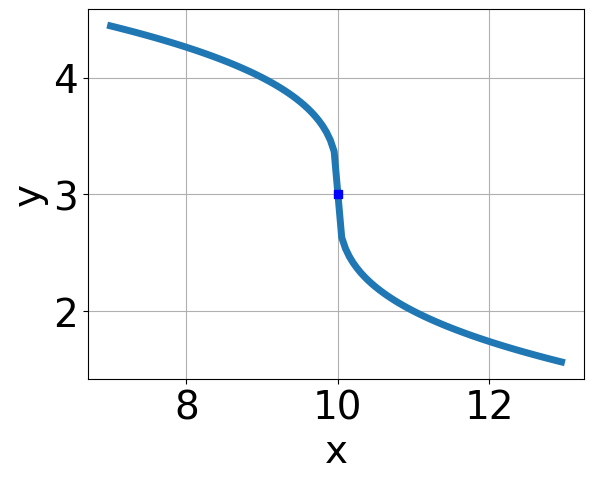
\includegraphics[width = 0.3\textwidth]{../Figures/radicalEquationToGraphCopyAA.png}\item 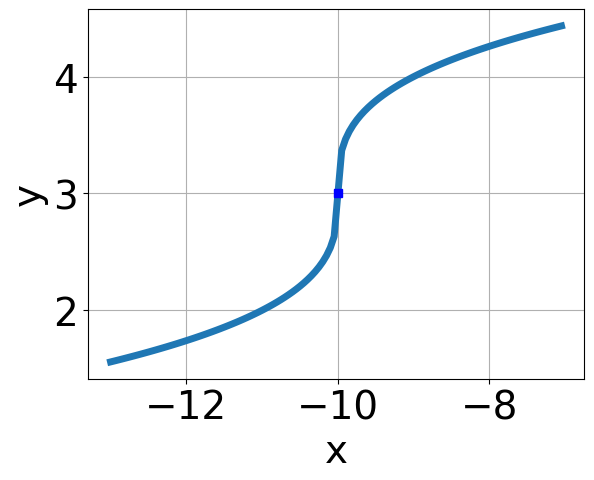
\includegraphics[width = 0.3\textwidth]{../Figures/radicalEquationToGraphCopyBA.png}\item 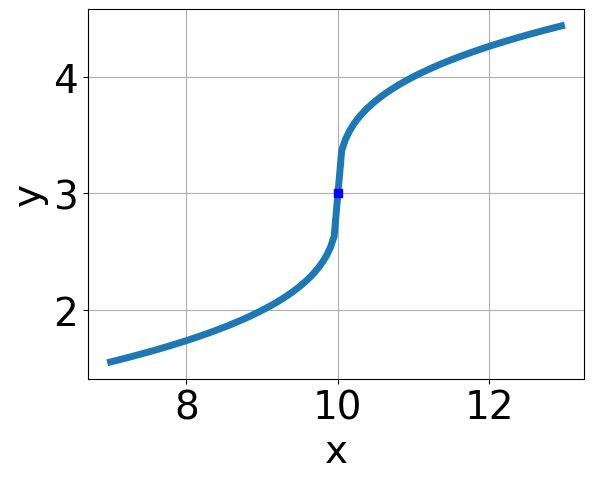
\includegraphics[width = 0.3\textwidth]{../Figures/radicalEquationToGraphCopyCA.png}\item 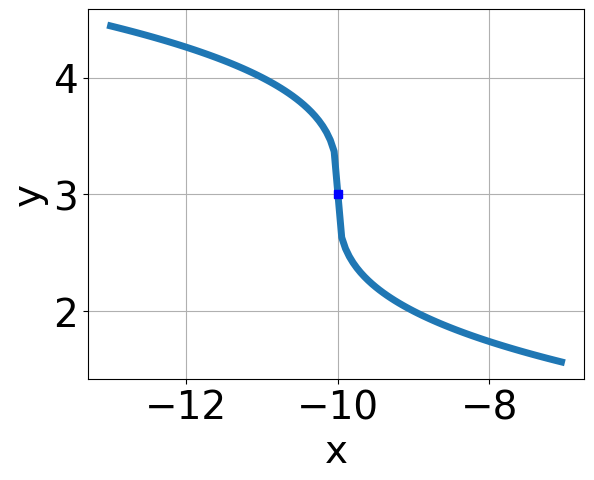
\includegraphics[width = 0.3\textwidth]{../Figures/radicalEquationToGraphCopyDA.png}\end{multicols}\item None of the above.
\end{enumerate} }
\litem{
Choose the equation of the function graphed below.
\begin{center}
    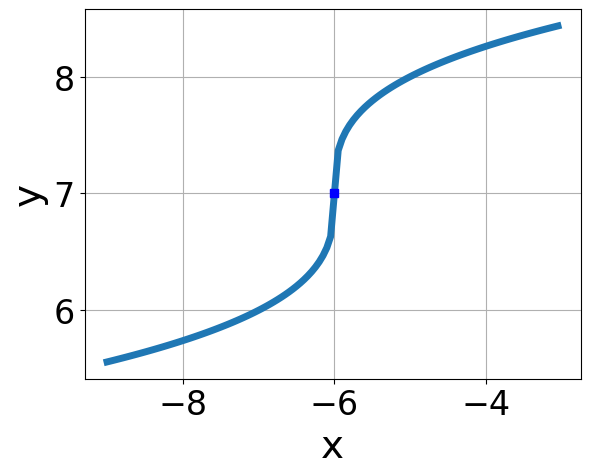
\includegraphics[width=0.5\textwidth]{../Figures/radicalGraphToEquationA.png}
\end{center}
\begin{enumerate}[label=\Alph*.]
\item \( f(x) = - \sqrt[3]{x + 6} + 7 \)
\item \( f(x) = - \sqrt[3]{x - 6} + 7 \)
\item \( f(x) = \sqrt[3]{x + 6} + 7 \)
\item \( f(x) = \sqrt[3]{x - 6} + 7 \)
\item \( \text{None of the above} \)

\end{enumerate} }
\litem{
Solve the radical equation below. Then, choose the interval(s) that the solution(s) belongs to.\[ \sqrt{-48 x^2 + 15} - \sqrt{-22 x} = 0 \]\begin{enumerate}[label=\Alph*.]
\item \( x_1 \in [0.37, 0.57] \text{ and } x_2 \in [-0.17,5.83] \)
\item \( x_1 \in [-0.55, -0.32] \text{ and } x_2 \in [-0.17,5.83] \)
\item \( \text{All solutions lead to invalid or complex values in the equation.} \)
\item \( x \in [-0.55,-0.32] \)
\item \( x \in [0.38,1.04] \)

\end{enumerate} }
\litem{
Solve the radical equation below. Then, choose the interval(s) that the solution(s) belongs to.\[ \sqrt{4 x - 7} - \sqrt{9 x - 2} = 0 \]\begin{enumerate}[label=\Alph*.]
\item \( x_1 \in [0.18, 0.79] \text{ and } x_2 \in [0.75,4.75] \)
\item \( x \in [-1.07,-0.45] \)
\item \( x_1 \in [-1.07, -0.45] \text{ and } x_2 \in [0.75,4.75] \)
\item \( \text{All solutions lead to invalid or complex values in the equation.} \)
\item \( x \in [-2.19,-1.77] \)

\end{enumerate} }
\litem{
What is the domain of the function below?\[ f(x) = \sqrt[3]{4 x + 3} \]\begin{enumerate}[label=\Alph*.]
\item \( \text{The domain is } (-\infty, a], \text{   where } a \in [-1.5, -1.33] \)
\item \( (-\infty, \infty) \)
\item \( \text{The domain is } (-\infty, a], \text{   where } a \in [-0.77, 0.93] \)
\item \( \text{The domain is } [a, \infty), \text{   where } a \in [-1.26, -0.5] \)
\item \( \text{The domain is } [a, \infty), \text{   where } a \in [-1.4, -1.33] \)

\end{enumerate} }
\litem{
Choose the graph of the equation below.\[ f(x) = \sqrt[3]{x + 10} - 7 \]\begin{enumerate}[label=\Alph*.]
\begin{multicols}{2}\item 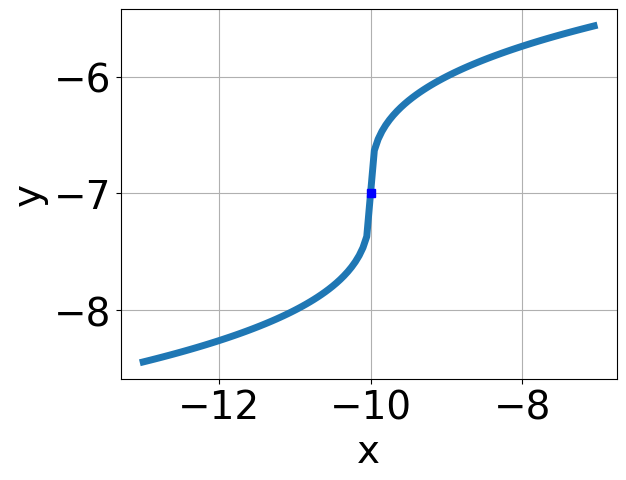
\includegraphics[width = 0.3\textwidth]{../Figures/radicalEquationToGraphAA.png}\item 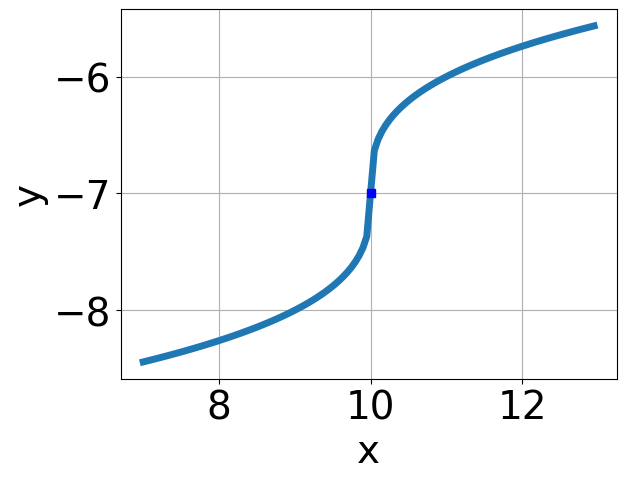
\includegraphics[width = 0.3\textwidth]{../Figures/radicalEquationToGraphBA.png}\item 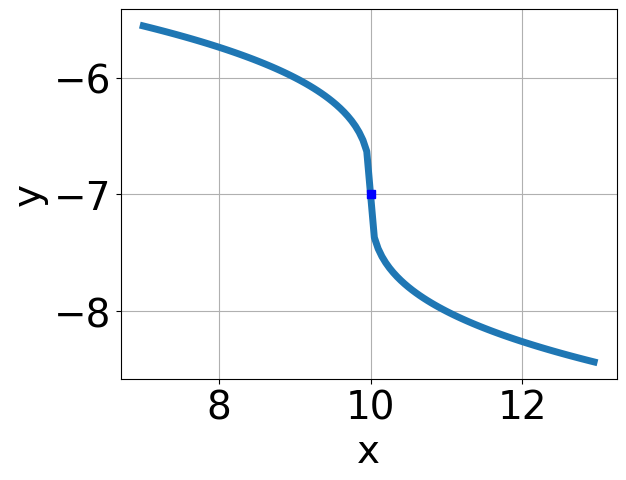
\includegraphics[width = 0.3\textwidth]{../Figures/radicalEquationToGraphCA.png}\item 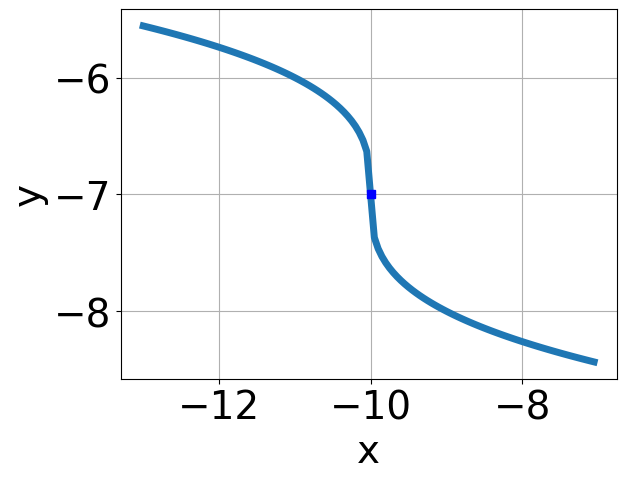
\includegraphics[width = 0.3\textwidth]{../Figures/radicalEquationToGraphDA.png}\end{multicols}\item None of the above.
\end{enumerate} }
\litem{
Choose the equation of the function graphed below.
\begin{center}
    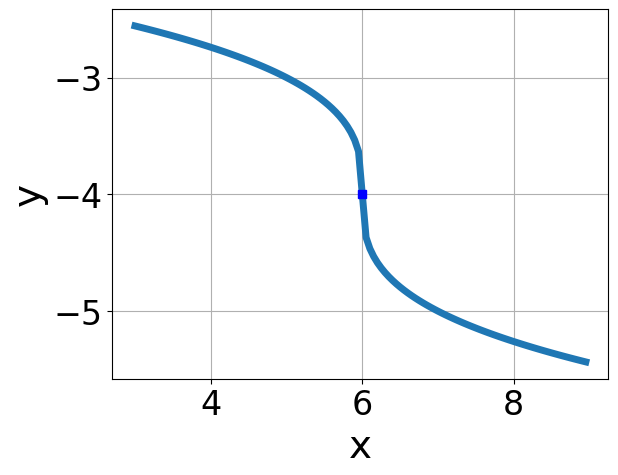
\includegraphics[width=0.5\textwidth]{../Figures/radicalGraphToEquationCopyA.png}
\end{center}
\begin{enumerate}[label=\Alph*.]
\item \( f(x) = - \sqrt{x - 6} - 4 \)
\item \( f(x) = - \sqrt{x + 6} - 4 \)
\item \( f(x) = \sqrt{x + 6} - 4 \)
\item \( f(x) = \sqrt{x - 6} - 4 \)
\item \( \text{None of the above} \)

\end{enumerate} }
\litem{
Solve the radical equation below. Then, choose the interval(s) that the solution(s) belongs to.\[ \sqrt{36 x^2 + 20} - \sqrt{-61 x} = 0 \]\begin{enumerate}[label=\Alph*.]
\item \( x \in [-1.86,-0.84] \)
\item \( \text{All solutions lead to invalid or complex values in the equation.} \)
\item \( x \in [-0.62,-0.28] \)
\item \( x_1 \in [-1.86, -0.84] \text{ and } x_2 \in [-1.9,-0.4] \)
\item \( x_1 \in [-0.31, 0.87] \text{ and } x_2 \in [1.2,2.2] \)

\end{enumerate} }
\litem{
What is the domain of the function below?\[ f(x) = \sqrt[6]{5 x + 3} \]\begin{enumerate}[label=\Alph*.]
\item \( (-\infty, a], \text{where } a \in [-1.15, 1.69] \)
\item \( (-\infty, \infty) \)
\item \( [a, \infty), \text{ where } a \in [-1.6, 5.4] \)
\item \( (-\infty, a], \text{where } a \in [-2.34, -1.3] \)
\item \( [a, \infty), \text{where } a \in [-4.67, -0.67] \)

\end{enumerate} }
\end{enumerate}

\end{document}